\documentclass{standalone}

\usepackage{tikz}

\begin{document}

	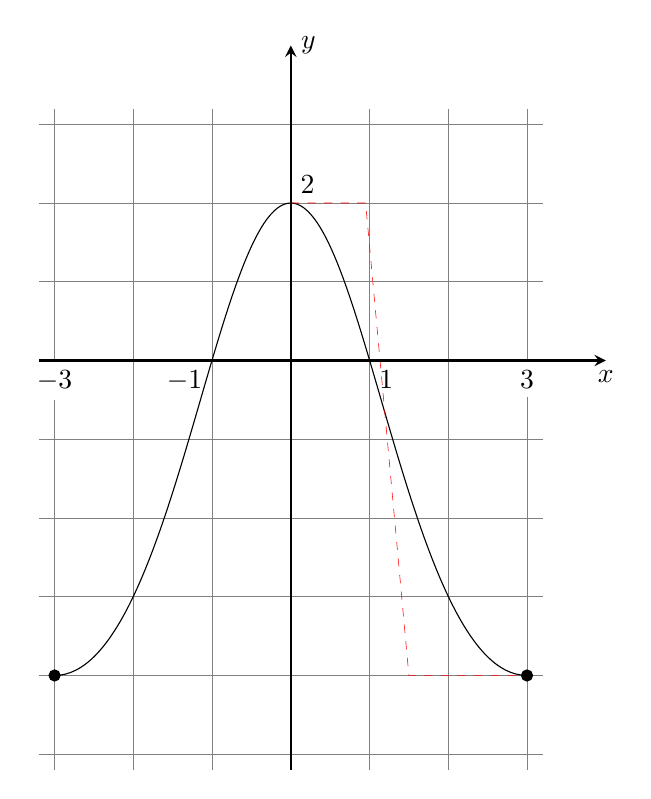
\begin{tikzpicture}[scale=1]
	
	\draw[step=1, very thin, color=gray] (-3.2,-5.2) grid (3.2,3.2);
	\coordinate (A) at (-3,-4);
	\coordinate (B) at (3,-4);
	\coordinate (C) at (0,2);
	
	\draw(C) .. controls (0.95,2) and (1.5,-4) .. (B);
	\draw[dashed, very thin, red] (C) -- (0.95,2) -- (1.5,-4) -- (B); 
	
	\draw(C) .. controls (-0.95,2) and (-1.5,-4) .. (A);
		
	\draw[radius=2pt,fill=black] (A) circle ;
	\draw[radius=2pt,fill=black] (B) circle ;
	
	\draw (-3,0) node[below, fill=white]{$-3$};
	\draw (3,0) node[below, fill=white]{$3$};
	\draw (0,2) node[above right]{$2$};
	\draw (-1,0) node[below left]{$-1$};
	\draw (1,0) node[below right]{$1$};
	\draw[thick, ->, >=stealth] (-3.2,0) -- (4,0) node[below]{\(x\)};
	\draw[thick, ->, >=stealth] (0,-5.2) -- (0,4) node[right]{$y$};

	\end{tikzpicture}

\end{document},